\documentclass[dvipsnames, tikz]{standalone}
\usepackage{amsmath}
\usepackage{arevmath}
\usepackage{xcolor}
\usepackage{tikz}
\usetikzlibrary{calc}
\usetikzlibrary{decorations.pathreplacing,calligraphy,3d}
\usetikzlibrary{matrix,shapes,fit,backgrounds}

\begin{document}
	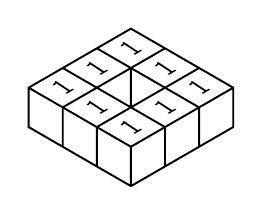
\begin{tikzpicture}[
		%Global config
		>=latex,
		line width=1pt,
		color = black,
		every left delimiter/.style={xshift=1ex},
		every right delimiter/.style={xshift=-1ex},
		%Styles
		Matrix/.style={
			matrix of nodes,
			column sep=1pt,
			row sep=1pt,
			nodes={draw=black!10}, % Uncoment to see the square nodes.
			%nodes in empty cells,
		},
		DA/.style={
			fill,
			opacity=0.2,
			rounded corners,
			inner sep=-3pt,
			line width=1pt,
		},
		main/.style={
			line width=0.7pt,
			color=black
			}
		]
			
		\begin{scope}[xshift=2cm, yshift=-1.5cm, scale=0.5, font=\small]
			\draw[main] (0,0) --++(30:3) --++(0,1) --++(150:3) --++(30:-3) --++(0,-1) --++(-30:3) (0,0) --++(0,1) --++(30:3) ++(30:-1) --++(150:3) ++(-30:1)++(30:1) --++(30:-3) ++(150:1) --++(-30:3) ++(30:1) --++(150:3) ++(0,-1) --++(0,-1) ++(-30:1) --++(0,1) --++(30:3) ++(0,-1) --++(0,-1) ++(30:-1) --++(0,1) ++(150:1) --++(0,1);
			\path (0,1.5) node[main, rotate=30,xslant=-0.5] {\sf 1};
			\path (30:1) ++ (0,1.5) node[main, rotate=30,xslant=-0.5] {\sf 1};
			\path (30:2) ++ (0,1.5) node[main, rotate=30,xslant=-0.5] {\sf 1};
			
			\path (30:1) ++ (0,2.5) node[main, rotate=30,xslant=-0.5] {\sf 1};
			
			\path (0,3.5) node[main, rotate=30,xslant=-0.5] {\sf 1};
			
			\path (-30:-1) ++ (0,1.5) node[main, rotate=30,xslant=-0.5] {\sf 1};
			\path (-30:-2) ++ (0,1.5) node[main, rotate=30,xslant=-0.5] {\sf 1};
			
			\path (-30:-1) ++ (0,2.5) node[main, rotate=30,xslant=-0.5] {\sf 1};
		\end{scope}
	\end{tikzpicture}
\end{document}